\documentclass[10pt]{article}

% Packages pour les marges
\usepackage[
    top=2cm,
    bottom=2cm,
    left=2cm,
    right=2cm
]{geometry}

% Police sans serif
% \usepackage{helvet}
% \renewcommand{\familydefault}{\sfdefault}

% Packages existants
\usepackage[french]{babel}
\usepackage[utf8]{inputenc}
\usepackage[T1]{fontenc}
\usepackage{amsmath}
\usepackage{amsfonts}
\usepackage{amssymb}
\usepackage[version=4]{mhchem}
\usepackage{stmaryrd}
\usepackage{xcolor}
\usepackage[cache=false]{minted}

\usemintedstyle{friendly}
\setminted[python]{
    frame=lines,
    framesep=2mm,
    baselinestretch=1.2,
    fontsize=\footnotesize,
    linenos=false,
    encoding=utf8
}

% Fix pour les caractères UTF-8 dans minted
\makeatletter
\AtBeginDocument{
  \def\MintedPygmentize{pygmentize -f latex -P encoding=utf8}
}
\makeatother

\usepackage{enumitem}
\usepackage{ifthen}
\usepackage{graphicx}
\usepackage{verbatim}
\usepackage{url}
\usepackage{mdframed}
\usepackage[sf]{titlesec}
\titleformat{\section}{\sffamily\large\bfseries}{\thesection}{1em}{}
% Définition de la variable pour afficher les corrections
\newboolean{showSolutions}
% Décommentez la ligne suivante pour afficher les solutions
\input \jobname.adr
% \input \jobname.adr


\title{TD4 - Analyse Numérique}

\author{}
\date{}

\newenvironment{solution}
    {\par\vspace{0.5em}\begin{mdframed}[linewidth=0.5pt]\par}
    {\end{mdframed}\par\vspace{0.5em}}

\begin{document}
\sffamily
\maketitle

\section*{Des polynômes dont on ne se lasse pas}
On souhaite approcher la fonction $f(x)=e^x$ sur l'intervalle $[0,12]$ par une fonction polynomiale par morceaux $\tilde{f}$ de la forme suivante : 
\[
\tilde{f}(x) = \begin{cases}
    P_1(x) & \text{si } x \in [0, 4] \\
    P_2(x) & \text{si } x \in [4, 8] \\
    P_3(x) & \text{si } x \in [8, 12]
\end{cases}
\]
avec $P_1$, $P_2$ et $P_3$ des polynômes de degré minimal et tels que $\tilde{f}(x)=f(x)$ pour $x=0, 2, 4, 6, 8, 10, 12$. 
\vspace{0.5em}

Déterminer $\tilde{f}(x)$ et tracer son graphe. 

\ifthenelse{\boolean{showSolutions}}{
    \begin{solution}
        Il faut procéder en 3 étapes, une pour chacun des intervalles. 


        \vspace{1em}

        Commençons par le polynôme qui va approcher la fonction sur l'intervalle $[0, 4]$. 
        On commence par construire les polynômes de Lagrange $L_0(x)$, $L_2(x)$ et $L_4(x)$ :
        \[
        L_0(x) = \frac{(x-2)(x-4)}{(0-2)(0-4)}, \qquad L_2(x) = \frac{x(x-4)}{2(2-4)}, \qquad L_4(x) = \frac{x(x-2)}{4(4-2)}
        \]
        On peut alors construire le premier polynôme :
        \[
        P_1(x) = 1L_0(x) + e^2 L_2(x) + e^4 L_4(x)
        \]

        \vspace{1em}

        Sur le deuxième intervalle, on construit les polynômes de Lagrange $L_4(x)$, $L_6(x)$ et $L_8(x)$ :
        \textbf{Attention, ce n'est pas le même $L_4$ que dans le premier intervalle !}
        \[
        L_4(x) = \frac{(x-6)(x-8)}{(4-6)(4-8)}, \qquad L_6(x) = \frac{(x-4)(x-8)}{(6-4)(6-8)}, \qquad L_8(x) = \frac{(x-4)(x-6)}{(8-4)(8-6)}
        \]
        On peut alors construire le deuxième polynôme :
        \[
        P_2(x) = e^4 L_4(x) + e^6 L_6(x) + e^8 L_8(x)
        \]

        \vspace{1em}

        On procède de la même façon pour le troisième intervalle. 
        On construit les polynômes de Lagrange $L_8(x)$, $L_{10}(x)$ et $L_{12}(x)$ :
        \[
        L_8(x) = \frac{(x-10)(x-12)}{(8-10)(8-12)}, \qquad L_{10}(x) = \frac{(x-8)(x-12)}{(10-8)(10-12)}, \qquad L_{12}(x) = \frac{(x-8)(x-10)}{(12-8)(12-10)}
        \]
        On peut alors construire le troisième polynôme :
        \[
        P_3(x) = e^8 L_8(x) + e^{10} L_{10}(x) + e^{12} L_{12}(x)
        \]

        Les graphes ne sont pas très faciles à tracer sur une même figure, cela nous montre aussi à quel point la fonction exponentielle grandit vite. 

        Nous séparons en deux images : la courbe exponentielle est la courbe bleue. 
        Sur l'intervalle $[0, 6]$, on a :
        \begin{center}
            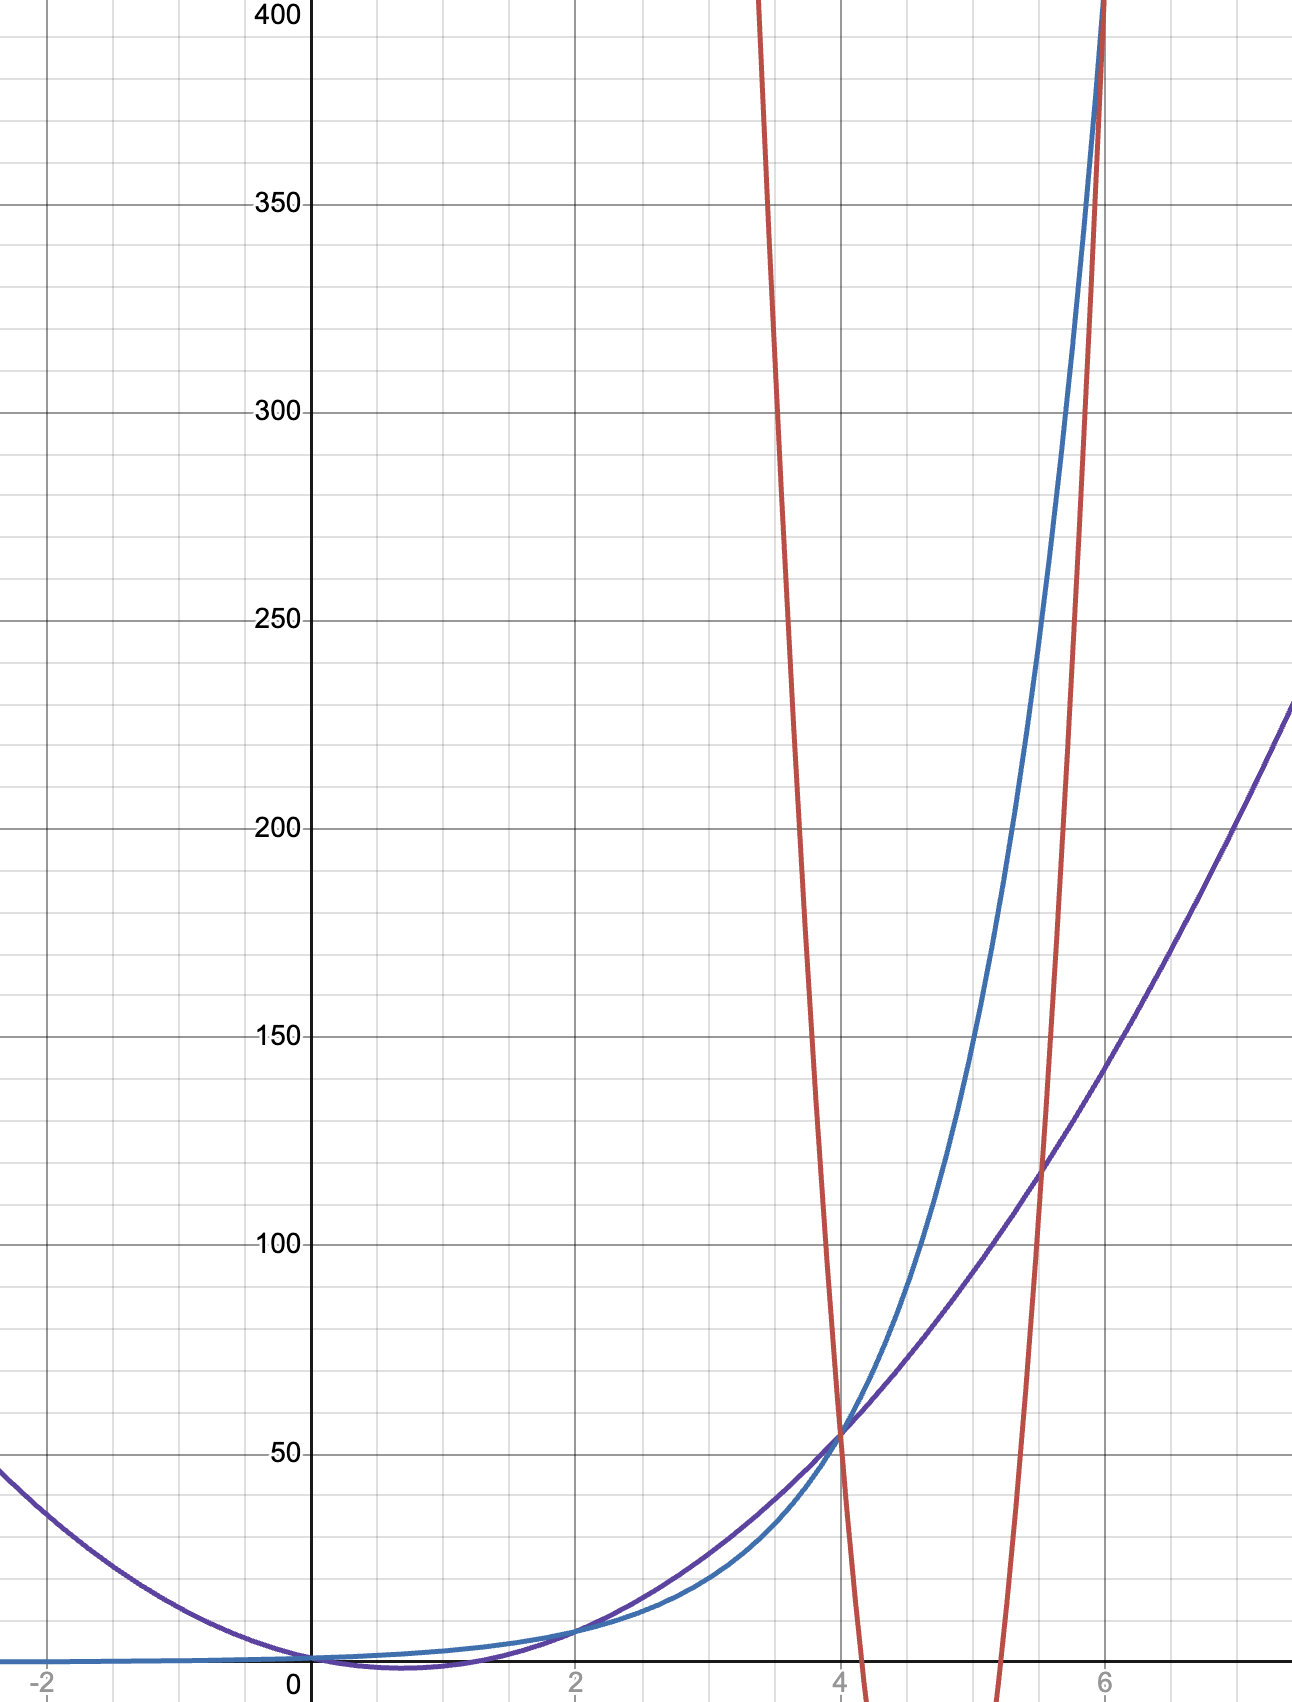
\includegraphics[width=0.8\textwidth]{graph1.png}
        \end{center}

        Sur l'intervalle $[6, 12]$, on a :
        \begin{center}
            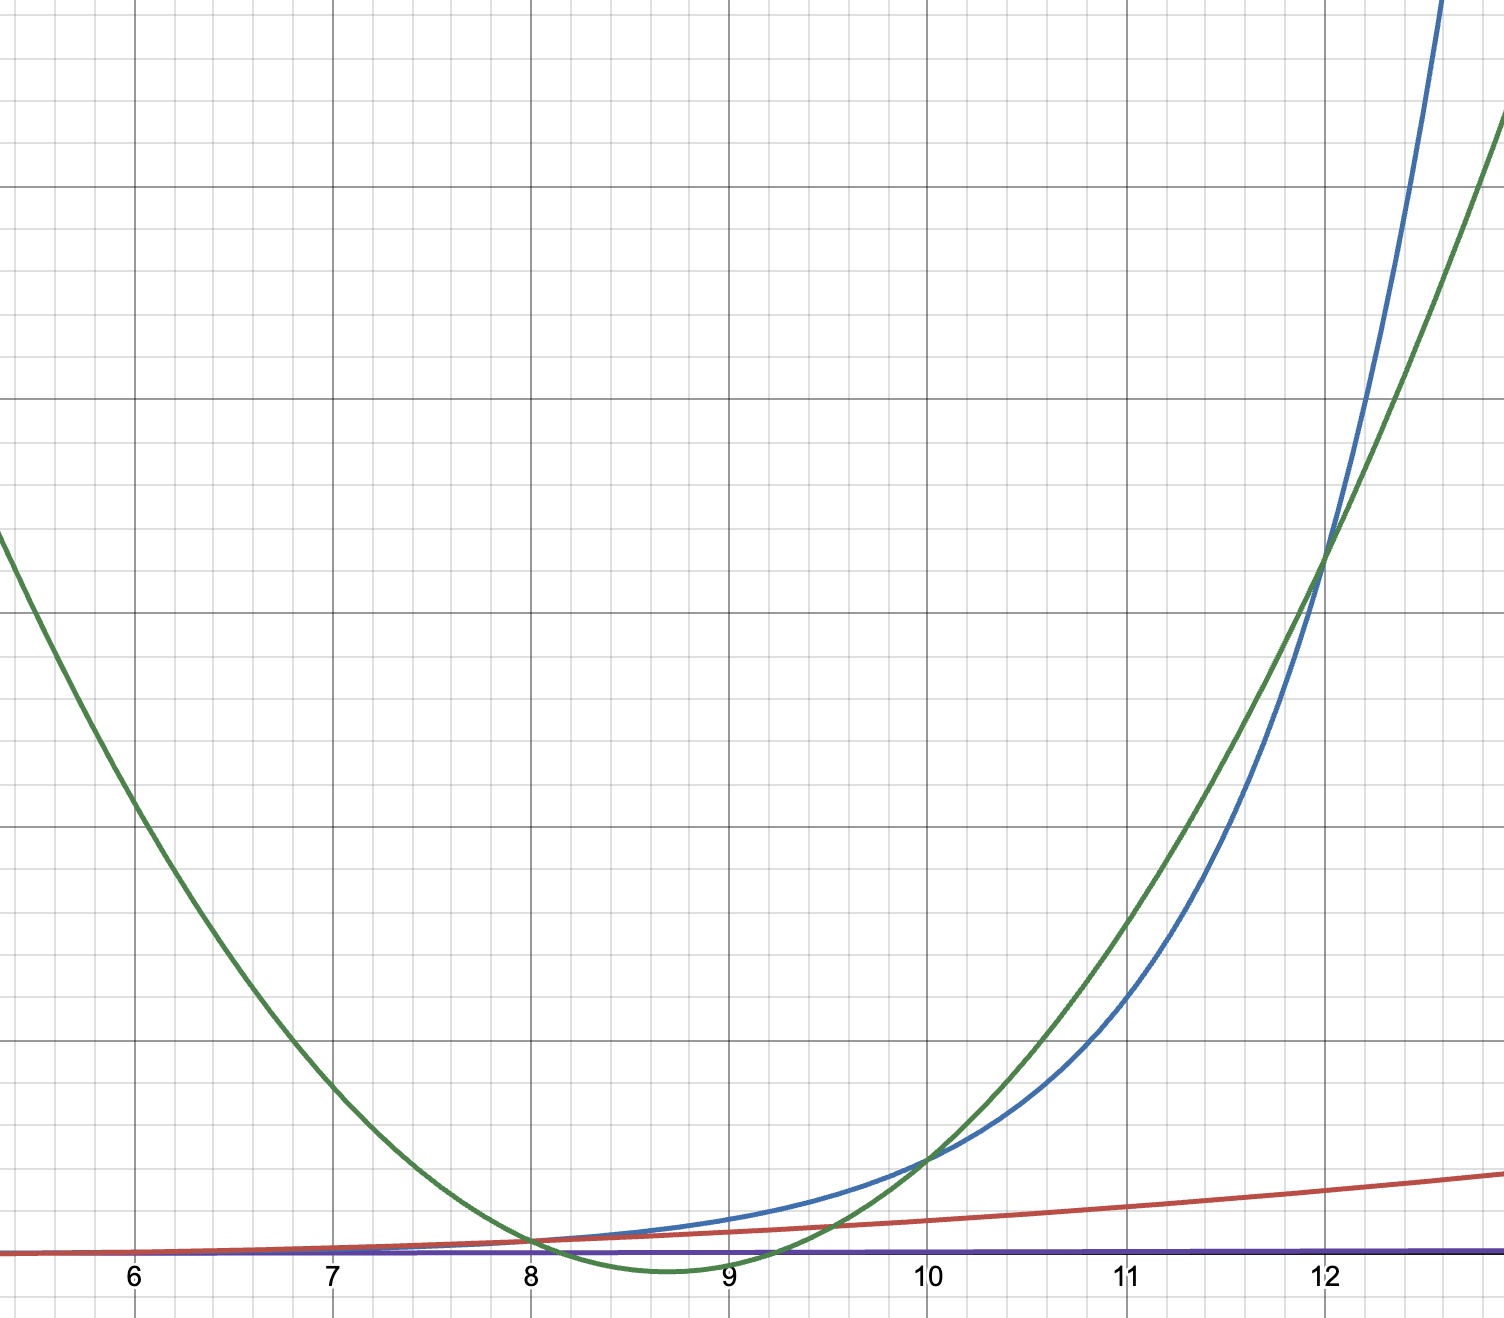
\includegraphics[width=0.8\textwidth]{graph2.png}
        \end{center}

    \end{solution}
}{}

\vspace{1cm}
\section*{Vers l'implémentation de la décomposition LU}

\begin{enumerate}
    \item Calculer la décomposition LU de la matrice $A=\left(\begin{array}{lll}4 & 1 & 1 \\ 2 & 5 & 1 \\ 1 & 1 & 6\end{array}\right)$.
    
    \ifthenelse{\boolean{showSolutions}}{
        \begin{solution}
            Les trois étapes à effectuer sont : 
            \[
            L_2 \leftarrow L_2 - \frac{1}{2} L_1
            \]
            \[
            L_3 \leftarrow L_3 - \frac{1}{4} L_1
            \]
            \[
            L_3 \leftarrow L_3 - \frac{1}{6} L_2
            \]
            On a donc $A = LU$ avec 
            \[
            L = \begin{pmatrix}
                1 & 0 & 0 \\
                1/2 & 1 & 0 \\
                1/4 & 1/6 & 1
            \end{pmatrix}
            \]
            et 
            \[
            U = \begin{pmatrix}
                4 & 1 & 1 \\
                0 & 9/2 & 1/2 \\
                0 & 0 & 17/3
            \end{pmatrix}
            \]
            
        \end{solution}
    }{}
    \item En déduire le déterminant de la matrice $A$. 

    \ifthenelse{\boolean{showSolutions}}{
        \begin{solution}
            On a $A = LU$ avec $L$ triangulaire inférieure et $U$ triangulaire supérieure. 
            Donc $\det(A) = \det(L) \det(U) = 4 \times \frac{9}{2} \times \frac{17}{3} = 102$. 
        \end{solution}
    }{}
    \vspace{1em}
    On cherche à écrire un algorithme qui calcule $L$ et $U$ à partir de $A$ sans effectuer l'algorithme de Gauss. 

    On écrit pour cela $A=LU$ avec $L$ triangulaire inférieure avec des $1$ sur la diagonale et $U$ triangulaire supérieure:
    \[
    A = \begin{pmatrix}
        a_{11} & a_{12} & a_{13} \\
        a_{21} & a_{22} & a_{23} \\
        a_{31} & a_{32} & a_{33}
    \end{pmatrix}
    = \begin{pmatrix}
        1 & 0 & 0 \\
        l_{21} & 1 & 0 \\
        l_{31} & l_{32} & 1
    \end{pmatrix}
    \begin{pmatrix}
        u_{11} & u_{12} & u_{13} \\
        0 & u_{22} & u_{23} \\
        0 & 0 & u_{33}
    \end{pmatrix}
    \]
    \item En écrivant le produit de la première ligne de $L$ par la matrice $U$, déterminer les $u_{1j}$.

    \ifthenelse{\boolean{showSolutions}}{
        \begin{solution}
            On obtient trois égalités : 
            \[
            u_{11} = a_{11}, \qquad u_{12} = a_{12}, \qquad u_{13} = a_{13}
            \]
        \end{solution}
    }{}

    \item En écrivant le produit de la matrice $L$ par la première colonne de $U$, déterminer les $l_{i1}$.

    \ifthenelse{\boolean{showSolutions}}{
        \begin{solution}
            La première égalité nous donne $u_{11}$ qu'on connait déjà, les deux autres donnent : 
            \[
            l_{21}u_{11} = a_{21}, \qquad l_{31}u_{11} = a_{31}
            \]
            On en déduit : 
            \[
            l_{21} = \frac{a_{21}}{u_{11}}, \qquad l_{31} = \frac{a_{31}}{u_{11}}
            \]
        \end{solution}
    }{}
    \item En écrivant le produit de la deuxième ligne de $L$ par la matrice $U$, déterminer les $u_{2j}$.

    \ifthenelse{\boolean{showSolutions}}{
        \begin{solution}
            On connait déjà $u_{11}$, les deux autres égalités donnent : 
            \[
            l_{21}u_{12} + u_{22} = a_{22} , \qquad l_{31}u_{12} + u_{23} = a_{23}
            \]
            On en déduit : 
            \[
            u_{22} = a_{22} - l_{21}u_{12}, \qquad u_{23} = a_{23} - l_{31}u_{12}
            \]
        \end{solution}
    }{}

    \item En écrivant le produit de la matrice $L$ par la deuxième colonne de $U$, déterminer les $l_{i2}$.

    \ifthenelse{\boolean{showSolutions}}{
        \begin{solution}
            Le dernier coefficient de la colonne donne 
            \[
            l_{31}u_{12} + l_{32}u_{22} = a_{32}
            \]
            donc 
            \[
            l_{32} = \frac{a_{32} - l_{31}u_{12}}{u_{22}}
            \]
        \end{solution}
    }{}
    \item En écrivant le produit de la troisième ligne de $L$ par la matrice $U$, déterminer les $u_{3j}$.

    \ifthenelse{\boolean{showSolutions}}{
        \begin{solution}
            Le coefficient 3eme ligne 3eme colonne donne  
            \[
            l_{31}u_{13} + l_{32}u_{23} + u_{33} = a_{33}
            \]
            on en déduit $u_{33}$ :
            \[
            u_{33} = a_{33} - l_{31}u_{13} - l_{32}u_{23}
            \]
        \end{solution}
    }{}
    \item Pour des matrices $n\times n$, donner les formules analogues pour $u_{1j}$ et $l_{i1}$, $u_{2j}$ et $l_{i2}$, $u_{3j}$ et $l_{i3}$.

    \ifthenelse{\boolean{showSolutions}}{
        \begin{solution}
            On obtient les formules suivantes : 
            \[
            u_{1j} = a{1j}, \qquad l_{i1} = \frac{a_{i1}}{u_{11}}\,.
            \]
            puis 
            \[
            u_{2j} = a_{2j} - l_{21}u_{1j}, \qquad l_{i2} = \frac{a_{i2} - l_{i1}u_{12}}{u_{22}}
            \]
            et enfin 
            \[
            u_{3j} = a_{3j} - l_{31}u_{1j} - l_{32}u_{2j}, \qquad l_{i3} = \frac{a_{i3} - l_{i1}u_{13} - l_{i2}u_{23}}{u_{33}}
            \]
        \end{solution}
    }{}
    \item Donner une formule générale pour $u_{ij}$ et $l_{ij}$ en fonction des valeurs de $A$ et des $u_{ik}$ et $l_{kj}$ pour $k<i$ et $k<j$.

    \ifthenelse{\boolean{showSolutions}}{
        \begin{solution}
            Les formules générales sont les suivantes : 
            \[
            u_{ij} = a_{ij} - \sum_{k=1}^{i-1} l_{ik}u_{kj}, \qquad l_{ij} = \frac{1}{u_{jj}}\Big(a_{ij} - \sum_{k=1}^{j-1} l_{ik}u_{kj}\Big)
            \]
        \end{solution}
    }{}
    \item En déduire un algorithme qui factorise une matrice $A$ en $A=LU$.

    \ifthenelse{\boolean{showSolutions}}{
        \begin{solution}
            Pour rédiger l'algorithme, il faut bien comprendre l'ordre dans lequel les calculs se font : 
            \begin{itemize}
                \item Les premiers termes qu'on peut calculer sont $u_{1j}$ et $l_{i1}$
                \item Ensuite, on peut calculer $u_{2j}$ et $l_{i2}$
                \item Enfin, on peut calculer $u_{3j}$ et $l_{i3}$
                \item ... 
            \end{itemize}
            Le programme consiste donc à faire une boucle. 

            Par exemple, le premier tour de boucle devra faire :

            \texttt{for j in range(n):}\\
            |\hspace{1em} \texttt{u[0,j] = a[0,j]}\\
            |\hspace{1em} \texttt{l[j,0] = a[j,0] / u[0,0]}

            Le second tour de boucle devra faire :

            \texttt{for j in range(n):}\\
            |\hspace{1em} \texttt{u[1,j] = a[1,j] - l[1,0] * u[0,j]}\\
            |\hspace{1em} \texttt{l[j,1] = (a[j,1] - l[j,0] * u[0,1]) / u[1,1]}

            Et ainsi de suite.

            On obtient par exemple l'algorithme suivant.
            On commence par initialiser $L$ et $U$ à la matrice nulle :

            \texttt{L = np.zeros((n,n))}\\
            \texttt{U = np.zeros((n,n))}

            On peut alors appliquer les formules précédentes :

            \texttt{for i in range(n):}\\
            |\hspace{1em} \texttt{for j in range(n):}\\
            |\hspace{1em} |\hspace{1em} \texttt{u[i,j] = a[i,j] - sum(l[i,k] * u[k,j] for k in range(j))}\\
            |\hspace{1em} |\hspace{1em} \texttt{l[j,i] = (a[j,i] - sum(l[j,k] * u[k,i] for k in range(j))) / u[i,i]}

            Ici, on a utilisé la fonction \texttt{sum} pour calculer de manière compacte les sommes nécessaires. 
        \end{solution}
    }{}
    \item Ecrire un algorithme qui donne la solution d'un système triangulaire supérieur, on lui donnera en paramètre une matrice $U$ triangulaire supérieure et un vecteur $b$, et il renverra le vecteur $x$ solution de $Ux=b$.

    \ifthenelse{\boolean{showSolutions}}{
        \begin{solution}
            Bien sûr, les coefficients diagonaux de $U$ ne sont pas nuls, sinon la matrice n'est pas inversible et le système n'admet pas de solution unique. 
            Pour résoudre un système triangulaire supérieur, on procède par étapes : 
            \begin{itemize}
                \item On commence par la dernière équation $u_{nn}x_n = b_n$ qui donne $x_n = b_n / u_{nn}$
                \item L'avant dernière équation s'écrit 
                \[
                u_{n-1,n-1}x_{n-1} + u_{n-1,n}x_n = b_{n-1}
                \]
                donc on en déduit $x_{n-1}$ :
                \[
                x_{n-1} = (b_{n-1} - u_{n-1,n}x_n) / u_{n-1,n-1}
                \]
                \item L'équation précédente s'écrit:
                \[
                u_{n-2,n-2}x_{n-2} + u_{n-2,n-1}x_{n-1} + u_{n-2,n}x_n = b_{n-2}
                \]
                donc on en déduit $x_{n-2}$ :
                \[
                x_{n-2} = (b_{n-2} - u_{n-2,n-1}x_{n-1} - u_{n-2,n}x_n) / u_{n-2,n-2}
                \]
                \item ...
            \end{itemize}
            L'algorithme est donc encore une boucle où chacun des tirets précédents correspond à une itération. Une solution est par exemple :

            \texttt{x = np.zeros(n)}\\
            \texttt{for i in range(n-1, -1, -1):}\\
            |\hspace{1em} \texttt{x[i] = (b[i] - sum(u[i,j] * x[j] for j in range(i+1,n))) / u[i,i]}
        \end{solution}
    }{}

    \item En utilisant les algorithmes précédents, écrire un algorithme qui calcule le déterminant d'une matrice $A$, un autre qui résout un système linéaire $Ax=b$ et un autre qui calcule l'inverse d'une matrice $A$.

    \ifthenelse{\boolean{showSolutions}}{
        \begin{solution}
            Si on appelle \texttt{getLU} et \texttt{solveTriSup} les fonctions précédentes, on peut écrire la fonction qui fait le produit des éléments diagonaux de $U$ :

            \texttt{L, U = getLU(A)}\\
            \texttt{np.prod(np.diag(U))}

            Et la fonction qui résout un système linéaire en introduisant la variable $Y = UX$ comme au TD précédent :

            \texttt{L, U = getLU(A)}\\
            \texttt{Y = solveTriInf(L, b)}\\
            \texttt{solveTriSup(U, Y)}

            Enfin, la fonction qui calcule l'inverse d'une matrice $A$ en introduisant la matrice $N = UM$ comme au TD précédent :

            \texttt{N = np.zeros((n,n))}\\
            \texttt{M = np.zeros((n,n))}
            \texttt{for i in range(n):}\\
            |\hspace{1em} \texttt{b = np.zeros(n)}\\
            |\hspace{1em} \texttt{b[i] = 1 \# b est la i-ième colonne de la matrice identité}\\
            |\hspace{1em} \texttt{N[:,i] = solveTriInf(L, b)}\\
            |\hspace{1em} \texttt{M[:,i] = solveTriSup(U, N[:,i])}
            \texttt{\# M est la matrice inverse de A}
        \end{solution}
    }{}

\end{enumerate}

\newpage

\section*{Variations sur la méthode de Jacobi}

\begin{enumerate}
    \item Rappelez le principe de la méthode de Jacobi. 

    \ifthenelse{\boolean{showSolutions}}{
        \begin{solution}
            La méthode de Jacobi est une méthode itérative pour résoudre un système linéaire $Ax=b$. 

            Elle ne donne pas la solution exacte, mais une solution approchée. Pour cela, on décompose $A$ en $A = D - E - F$ avec $D$ diagonale, $E$ triangulaire inférieure et $F$ triangulaire supérieure. 
            
            On peut alors réécrire le système $Ax=b$ sous la forme équivalente : 
            \[
            x = D^{-1}(b + (E + F)x)
            \]
            On choisit ensuite une valeur initiale $x^{(0)}$ et on itère la formule précédente : 
            \[
            x^{(k+1)} = D^{-1}(b + (E + F)x^{(k)})
            \]
            On peut montrer que la méthode converge si $A$ est diagonalement dominante. 
        \end{solution}
    }{}

    \item Plutôt que de décomposer une matrice $A$ en $A = D - E - F$, on peut la décomposer en $A = L + U$ avec $L$ triangulaire inférieure et $U$ triangulaire supérieure. \newline
    Montrer que la solution du système $Ax=b$ vérifie 
    \[
    X = L^{-1}\left(b-Ux\right).
    \]
    \ifthenelse{\boolean{showSolutions}}{
        \begin{solution}
            On a $A = L + U$ donc $Ax = (L + U)x = b$ donc $Lx + Ux = b$ donc $x = L^{-1}(b - Ux)$.
        \end{solution}
    }{}

    \item Déterminer une méthode itérative basée sur cette équation pour obtenir une solution approchée du système $Ax=b$. 
    \textit{On l'appelle la méthode de Gauss-Seidel, elle converge sous les mêmes conditions que la méthode de Jacobi.}

    \ifthenelse{\boolean{showSolutions}}{
        \begin{solution}
            On choisit une valeur initiale $x^{(0)}$ et on itère la formule précédente : 
            \[
            x^{(k+1)} = L^{-1}(b - Ux^{(k)})
            \]
        \end{solution}
    }{}
    \item Appliquer cette méthode au système $Ax=b$ avec $A=\left(\begin{array}{lll}4 & 1 & 1 \\ 2 & 5 & 1 \\ 1 & 1 & 6\end{array}\right)$ et $b=\left(\begin{array}{c}9 \\ 15 \\ 21\end{array}\right)$.

    \ifthenelse{\boolean{showSolutions}}{
        \begin{solution}
            On part par exemple du point $x^{(0)} = (1,1,1)$.
            Les équations qui décrivent l'évolution de $x^{(k)}$ sont : 
            \[
            \begin{aligned} 
                x_1^{(k+1)}& =\frac{1}{4}\left(9-x_2^{(k)}-x_3^{(k)}\right) \\ 
                x_2^{(k+1)}& =\frac{1}{5}\left(15-2 x_1^{(k+1)}-x_3^{(k)}\right) \\ 
                x_3^{(k+1)}& =\frac{1}{6}\left(21-x_1^{(k+1)}-x_2^{(k+1)}\right)
            \end{aligned}
            \]
            
            Les 5 premières itérations sont 
            \[
            \begin{aligned} 
                & x^{(0)}=(1.0000,1.0000,1.0000) \\ 
                & x^{(1)}=(1.7500,2.4000,3.1667) \\ 
                & x^{(2)}=(0.8583,1.6667,2.8083) \\ 
                & x^{(3)}=(1.1313,2.0950,3.0792) \\ 
                & x^{(4)}=(0.9565,1.9317,2.9623)
            \end{aligned}
            \]

            On observe la convergence vers la solution exacte $(1,2,3)$.
        \end{solution}
    }{}

    \item Concrètement, quelles sont les différences entre la méthode de Jacobi et la méthode de Gauss-Seidel ? 

    \ifthenelse{\boolean{showSolutions}}{
        \begin{solution}
            La méthode de Jacobi met à jour toutes les composantes de $x^{(k+1)}$ d'un coup, alors que la méthode de Gauss-Seidel met à jour les composantes de $x^{(k+1)}$ une par une et utilise les valeurs mises à jour.
            On pourrait donc penser que la méthode de Gauss-Seidel converge plus vite que la méthode de Jacobi. 
            
            En revanche la méthode de Gauss-Seidel demande de calculer $L^{-1}$ et donc de faire plus de calculs si $n$ est grand. 
        \end{solution}
    }{}
   
    \item Ecrivez un algorithme qui calcule la solution approchée d'un système linéaire $Ax=b$ en utilisant la méthode de Gauss-Seidel.

    \ifthenelse{\boolean{showSolutions}}{
        \begin{solution}
            On part d'un vecteur $x^{(0)}$ et on itère la formule : 
            \[
            x^{(k+1)} = L^{-1}(b - Ux^{(k)})
            \]
            On peut écrire l'algorithme suivant: On commence par construire les matrices $L$ et $U$, on utilise le programme de l'exercice précédent pour calculer $L^{-1}$, puis on itère la formule.
            
            \texttt{x = np.zeros(n)}\\
            \texttt{for k in range(100):}\\
            |\hspace{1em} \texttt{x = L\_inv @ (b - U @ x)}
        \end{solution}
    }{}
\end{enumerate}

\vspace{1em}
\section*{Calculer des solutions approchées d'équations différentielles}

    Si vous ne l'avez pas encore fait, lisez l'exercice \textbf{Vers la résolution des équations différentielles} du TD 3. 

    Prenons le problème de Cauchy suivant défini sur l'intervalle $[0,1]$: 
    \[
    \begin{cases}
        y' = f(t,y) \\
        y(0) = y_0
    \end{cases}
    \]

    Dans l'exercice du TD 3, nous avons écrit ce problème sous une forme discrétisée: une solution $y$ est approchée par une liste de points $(t_i,y_i)$ qui vérifient 
    \[
    y_{i+1} - y_i = \int_{t_i}^{t_{i+1}} f(t,y(t)) dt
    \]
    Ce genre de méthode pour obtenir une solution approchée d'une équation différentielle est appelée \textbf{méthode des différences finies}. 

    \begin{enumerate}
        \item En utilisant la méthode des rectangles à gauche, écrire un algorithme qui calcule les $y_i$ à partir de $y_0$ et de $f$.\newline
        \textit{Cette méthode permettra de calculer explicitement $y_{i+1}$ en fonction de $y_i$ et de $f$, on l'appelle la méthode d'Euler explicite.}

        \ifthenelse{\boolean{showSolutions}}{
            \begin{solution}
                On écrit la formule de la méthode des rectangles à gauche : 
                \[
                y_{i+1} - y_i = \int_{t_i}^{t_{i+1}} f(t,y(t)) dt = f(t_i,y(t_i))(t_{i+1}-t_i)
                \]
                On peut approcher $y(t_i)$ par $y_i$ et donc écrire : 
                \[
                y_{i+1} = y_i + f(t_i,y_i)(t_{i+1}-t_i)
                \]
                On peut donc écrire l'algorithme suivant : 
                \texttt{t = np.linspace(0,1,n+1)}\\
                \texttt{y = np.zeros(n+1)}\\
                \texttt{y[0] = y0}\\
                \texttt{for i in range(n):}\\
                |\hspace{1em} \texttt{y[i+1] = y[i] + f(t[i], y[i]) * (t[i+1] - t[i])}
            \end{solution}
        }{}

        \item En utilisant la méthode des rectangles à droite, écrire un algorithme qui calcule les $y_i$ à partir de $y_0$ et de $f(t, y) = q y$, $q$ étant une constante réelle.\newline
        \textit{Cette méthode ne donnera pas $y_{i+1}$ directement. Il faudra encore résoudre une équation pour trouver $y_{i+1}$, on l'appelle la méthode d'Euler implicite.}

        \ifthenelse{\boolean{showSolutions}}{
            \begin{solution}
                La méthode des rectangles à droite donne : 
                \[
                y_{i+1} - y_i = \int_{t_i}^{t_{i+1}} f(t,y(t)) dt = f(t_{i+1},y_{i+1})(t_{i+1}-t_i)
                \]
                On peut approcher $y(t_{i+1})$ par $y_{i+1}$ et donc écrire : 
                \[
                y_{i+1} = y_i + f(t_{i+1},y_{i+1})(t_{i+1}-t_i)
                \]
                en remplaçant $f$ par $q y$ on obtient : 
                \[
                y_{i+1} = y_i + q y_{i+1}(t_{i+1}-t_i)
                \]
                La relation qui permet de calculer $y_{i+1}$ en fonction de $y_i$ est donc : 
                \[
                y_{i+1} = \frac{y_i}{1-q(t_{i+1}-t_i)}
                \]
                On peut donc écrire l'algorithme suivant : 
                \texttt{y = np.zeros(n+1)}\\
                \texttt{y[0] = y0}\\
                \texttt{for i in range(n):}\\
                |\hspace{1em} \texttt{y[i+1] = y[i] / (1 - q * (t[i+1] - t[i]))}
            \end{solution}
        }{}
        \item En utilisant la méthode des trapèzes, écrire un algorithme qui calcule les $y_i$ à partir de $y_0$ et de $f(t, y) = q y$, $q$ étant une constante réelle..\newline 
        \textit{Cette méthode nécessitera aussi de résoudre une équation pour trouver $y_{i+1}$, c'est la méthode de Crank Nicolson}

        \ifthenelse{\boolean{showSolutions}}{
            \begin{solution}
                La méthode des trapèzes donne : 
                \[
                y_{i+1} - y_i = \int_{t_i}^{t_{i+1}} f(t,y(t)) dt = \frac{f(t_i,y_i) + f(t_{i+1},y_{i+1})}{2}(t_{i+1}-t_i)
                \]
                En remplaçant $f$ par $q y$ on obtient : 
                \[
                y_{i+1} - y_i = \frac{q y_i + q y_{i+1}}{2}(t_{i+1}-t_i)
                \]
                La relation qui permet de calculer $y_{i+1}$ en fonction de $y_i$ est donc : 
                \[
                y_{i+1} = y_i\, \frac{1+q(t_{i+1}-t_i)/2}{1-q(t_{i+1}-t_i)/2}
                \]
                On peut donc écrire l'algorithme suivant : 
                \texttt{y = np.zeros(n+1)}\\
                \texttt{y[0] = y0}\\
                \texttt{for i in range(n):}\\
                |\hspace{1em} \texttt{y[i+1] = y[i] * (1 + q * (t[i+1] - t[i]) / 2) / (1 - q * (t[i+1] - t[i]) / 2)}
            \end{solution}
        }{}
        \item Ces méthodes vont-elles converger vers la solution exacte ? 

        \ifthenelse{\boolean{showSolutions}}{
            \begin{solution}
                Il faut étudier la convergence lorsque le pas de temps tend vers $0$, c'est-à-dire lorsque $t_{i+1}-t_i$ tend vers $0$.
                Pour montrer cette convergence, il faut étudier $y(t_{i})-y_i$.

                On peut calculer la solution exacte de l'équation différentielle : 
                \[
                y(t) = y_0 e^{q t}
                \]
                De plus, la première méthode (Euler explicite) donne : 
                \[
                y_{i+1} = y_i + q y_i (t_{i+1}-t_i)
                \]
                C'est une relation de récurrence qu'on peut résoudre, en notant $h = t_{i+1}-t_i$ :  
                \[
                y_n = y_0 (1+qh)^n
                \]
                On peut donc écrire lorsque $h$ tend vers $0$ : 
                \[
                y_i = y_0 \exp\Big(n \ln(1+qh)\Big) = y_0 \exp(nqh + o(h))
                \]

                Ainsi, 
                \[
                y(t_n) - y_n = y(nh) - y_n = y_0 \exp(nqh) - y_0 \exp(nqh + o(h)) = y_0 o(h)
                \]
                On peut donc conclure que la méthode d'Euler explicite converge vers la solution exacte lorsque $h$ tend vers $0$.

                On peut procéder de la même façon avec les autres méthodes.
            \end{solution}
        }{}

        \item En utilisant la formule de quadrature de Newton Cotes, écrire un algorithme qui calcule les $y_i$ à partir de $y_0$ et de $f(t, y) = q y$, $q$ étant une constante réelle.\newline
        \textit{Cette méthode nécessitera de résoudre une équation pour trouver $y_{i+1}$, on l'appelle la méthode de Runge Kutta d'ordre 2.}

        \ifthenelse{\boolean{showSolutions}}{
            \begin{solution}
                La formule de quadrature de Newton Cotes donne : 
                \[
                \int_{t_i}^{t_{i+1}} f(t,y(t)) dt = \frac{t_{i+1}-t_i}{6}\Big(f(t_i,y_i) + 4f\big(\frac{t_i+t_{i+1}}{2}, \frac{y_i+y_{i+1}}{2}\big) + f(t_{i+1},y_{i+1})\Big)
                \]
                En remplaçant $f$ par $q y$ on obtient : 
                \[
                y_{i+1} - y_i = (t_{i+1}-t_i)\frac{q y_i + q y_{i+1}}{2}
                \]
                Pour cette fonction spécifiquement, on se ramène donc au cas précédent, la méthode de Newton-Cotes, qui permet d'obtenir une meilleure approximation de l'intégrale, ne conduit pas à une méthode plus précise ici. 
    
            \end{solution}
        }{}

    \end{enumerate}
    

\end{document}
